% Quatre isomères de formule brute C4H10O (exercice 4, chapitre 11)
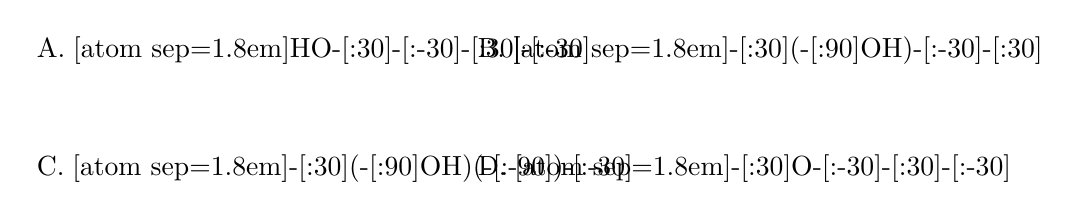
\begin{tikzpicture}[x=1cm,y=1cm]
\node[anchor=west] at (0,1.9) {\otLabel{A.}\;\chemfig[atom sep=1.8em]{HO-[:30]-[:-30]-[:30]-[:-30]}};
\node[anchor=west] at (5.6,1.9) {\otLabel{B.}\;\chemfig[atom sep=1.8em]{-[:30](-[:90]OH)-[:-30]-[:30]}};
\node[anchor=west] at (0,0.4) {\otLabel{C.}\;\chemfig[atom sep=1.8em]{-[:30](-[:90]OH)(-[:-90])-[:-30]}};
\node[anchor=west] at (5.6,0.4) {\otLabel{D.}\;\chemfig[atom sep=1.8em]{-[:30]O-[:-30]-[:30]-[:-30]}};
\end{tikzpicture}
\par\smallskip\legende{Quatre molécules de formule brute C$_4$H$_{10}$O.}
